% Ci sono iniziative che per l'enabling di calcolo numerico anche complesso sul client web
% poi spiego il modo
%% spiego da dove arriva
%% immagine di come funziona (plugin)

With the advent of \ac{GPGPU}, the spreading of multicore CPUs and multiprocessor
programming (like OpenMP) we can see emerging an intersection in parallel computing.
This intersection is known as \textbf{heterogeneus computing}. There are
initiatives aimed at enabling numeric calculation, even complex, on the web client.
\ac{OpenCL} is a framework for heterogeneus computing and \ac{WebCL} is a porting
of this technlogy to the web.\\
% Spiego meglio perchè è nato?

\begin{figure}[htb]
    \centering
    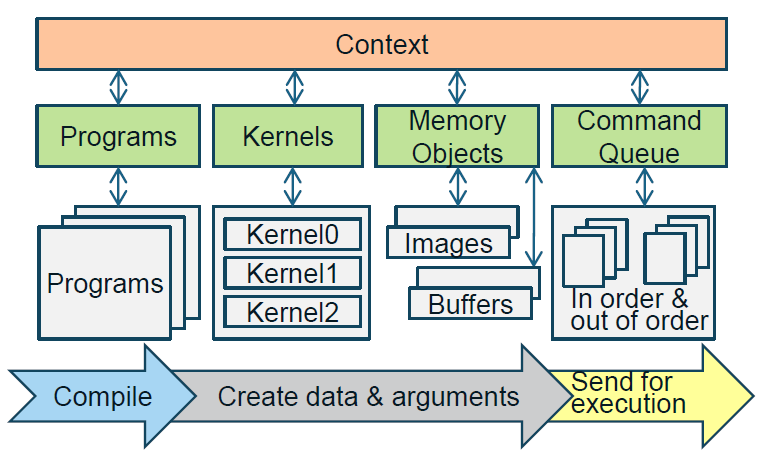
\includegraphics[width=\columnwidth]{opencl}
    \caption{OpenCL execution flow.}
    \label{fig:opencl}
\end{figure}
\ac{OpenCL} uses a language based on C99\footnote{A programming language dialect
for the past C developed in 1999 (formal name ISO/IEC 9899:1999)} for writing
\emph{kernels}, functions that actually execute on OpenCL devices. Here is the
list of action performed to run code on \ac{OpenCL} enabled computers:
\begin{enumerate}
    \item Query host for OpenCL devices.
    \item Create a context to associate OpenCL devices.
    \item Create programs for execution on one or more associated devices.
    \item From the programs, select kernels to execute.
    \item Create memory objects accessible from the host and/or the device.
    \item Copy memory data to the device as needed.
    \item Provide kernels to the command queue for execution.
    \item Copy results from the device to the host
\end{enumerate}


% TODO rifati? togli?
The main focus when building high-end web-application like 3D games is
responsiveness. Altough \js{} can be optimized and parallelized (see
\ref{sec:bg:web:html5}) it cannot be fast as an application software, because
\js{} must be interpreted by the browser and then executed as machine code.
\ac{WebCL} provide an easy framework for building and running machine code in
parallel directly from the browser.

% Implementazioni
%% common API 
% prestazioni, esempi
% integrazione con webGL
